\section{Natural Numbers}

\subsection{Peano Models}

In this section, we introduce the set of natural numbers and construct them using fundamental axioms of set theory. Before we construct the natural numbers, we can already make statements about the structure that the natural numbers are intended to satisfy. The structure of the natural numbers is defined by the so-called Peano axioms:

\begin{definition}[Peano Models]
    Let $N$ be a set, $0$ a distinct element of $N$, and $\sigma\colon N\rightarrow N\setminus\{0\}$ a mapping. Then the triple $(N,0,\sigma)$ is called a \emph{Peano model} if and only if the following \emph{Peano axioms} are satisfied:
    \begin{definitionenumerate}[label=\bfseries(P\arabic*),ref=\thedefinition(P\arabic*)]
        \item\label{definition:natural_numbers:peano_axiom_injective} $\sigma$ is injective.
        \item\label{definition:natural_numbers:peano_axiom_induction} For every subset $S\subseteq N$ with $0\in S$ and $\sigma(n)\in S$ for every $n\in N$ follows $S=N$.
    \end{definitionenumerate}
    If $(N,0,\sigma)$ is a Peano model, then $\sigma$ is referred to as the \emph{successor function}. For each $n\in N$, let $\sigma(n)$ denote the \emph{successor of $n$}. Axiom (P2) is also known as the \emph{induction axiom}.
\end{definition}

\begin{figure}[ht]
    \centering

    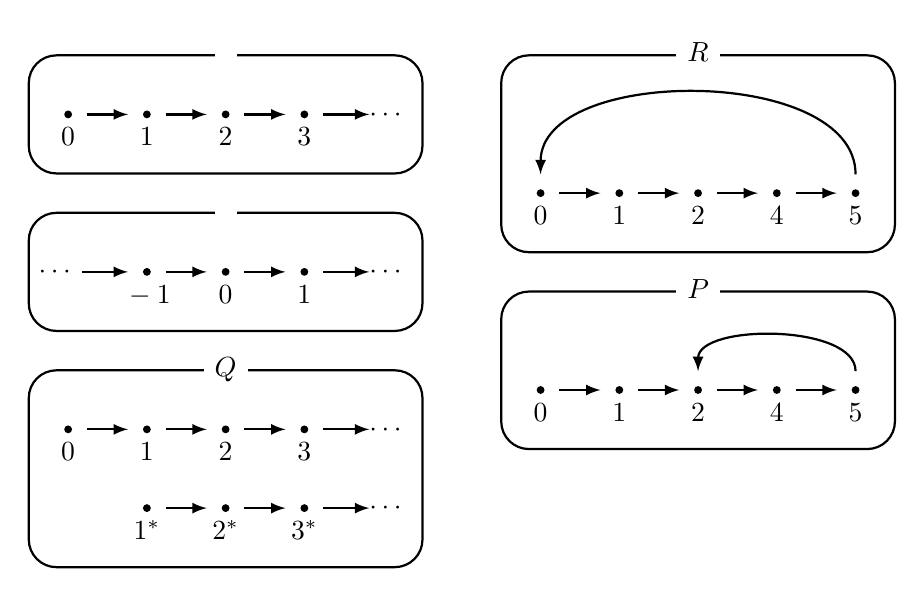
\begin{tikzpicture}[
        dot/.style={circle,fill=black,inner sep=1pt},
        element/.style={rectangle,fill=white,inner sep=0pt,outer sep=3pt},
        arrow/.style={-latex,shorten >=5pt,shorten <=5pt},
        curved arrow/.style={-latex,shorten >=5pt,shorten <=5pt,out=90,in=90},
        set/.style={rounded corners=10pt},
        set annotator/.style={fill=white,inner sep=4pt,rectangle},
        thick
    ]

    \begin{scope}[shift={(0,3)}]
        \coordinate[dot] (a-0) at (0,0);
        \coordinate[dot] (a-1) at (1,0);
        \coordinate[dot] (a-2) at (2,0);
        \coordinate[dot] (a-3) at (3,0);
        \coordinate[] (a-4) at (4,0);
        \draw[set] (-.5,-.75) rectangle (4.5,.75);
        \node[set annotator] at (2,.75) {$\strut \setN$};
    \end{scope}

    \node[element,below] at (a-0) {$\strut 0$};
    \node[element,below] at (a-1) {$\strut 1$};
    \node[element,below] at (a-2) {$\strut 2$};
    \node[element,below] at (a-3) {$\strut 3$};
    \node[element] at (a-4) {$\strut \cdots$};

    \draw[arrow] (a-0) to (a-1);
    \draw[arrow] (a-1) to (a-2);
    \draw[arrow] (a-2) to (a-3);
    \draw[arrow] (a-3) to (a-4);

    \begin{scope}[shift={(0,1)}]
        \coordinate[] (a-0) at (0,0);
        \coordinate[dot] (a-1) at (1,0);
        \coordinate[dot] (a-2) at (2,0);
        \coordinate[dot] (a-3) at (3,0);
        \coordinate[] (a-4) at (4,0);
        \draw[set] (-.5,-.75) rectangle (4.5,.75);
        \node[set annotator] at (2,.75) {$\strut \setZ$};
    \end{scope}

    \node[element,left=-4pt] at (a-0) {$\strut \cdots$};
    \node[element,below] at (a-1) {$\strut -1$};
    \node[element,below] at (a-2) {$\strut 0$};
    \node[element,below] at (a-3) {$\strut 1$};
    \node[element] at (a-4) {$\strut \cdots$};

    \draw[arrow] (a-0) to (a-1);
    \draw[arrow] (a-1) to (a-2);
    \draw[arrow] (a-2) to (a-3);
    \draw[arrow] (a-3) to (a-4);

    \begin{scope}[shift={(6,2)}]
        \coordinate[dot] (a-0) at (0,0);
        \coordinate[dot] (a-1) at (1,0);
        \coordinate[dot] (a-2) at (2,0);
        \coordinate[dot] (a-3) at (3,0);
        \coordinate[dot] (a-4) at (4,0);
        \draw[set] (-.5,-.75) rectangle (4.5,1.75);
        \node[set annotator] at (2,1.75) {$\strut R$};
    \end{scope}

    \node[element,below] at (a-0) {$\strut 0$};
    \node[element,below] at (a-1) {$\strut 1$};
    \node[element,below] at (a-2) {$\strut 2$};
    \node[element,below] at (a-3) {$\strut 3$};
    \node[element,below] at (a-3) {$\strut 4$};
    \node[element,below] at (a-4) {$\strut 5$};

    \draw[arrow] (a-0) to (a-1);
    \draw[arrow] (a-1) to (a-2);
    \draw[arrow] (a-2) to (a-3);
    \draw[arrow] (a-3) to (a-4);
    \draw[curved arrow] (a-4) to (a-0);

    \begin{scope}[shift={(6,-.5)}]
        \coordinate[dot] (a-0) at (0,0);
        \coordinate[dot] (a-1) at (1,0);
        \coordinate[dot] (a-2) at (2,0);
        \coordinate[dot] (a-3) at (3,0);
        \coordinate[dot] (a-4) at (4,0);
        \draw[set] (-.5,-.75) rectangle (4.5,1.25);
        \node[set annotator] at (2,1.25) {$\strut P$};
    \end{scope}

    \node[element,below] at (a-0) {$\strut 0$};
    \node[element,below] at (a-1) {$\strut 1$};
    \node[element,below] at (a-2) {$\strut 2$};
    \node[element,below] at (a-3) {$\strut 3$};
    \node[element,below] at (a-3) {$\strut 4$};
    \node[element,below] at (a-4) {$\strut 5$};

    \draw[arrow] (a-0) to (a-1);
    \draw[arrow] (a-1) to (a-2);
    \draw[arrow] (a-2) to (a-3);
    \draw[arrow] (a-3) to (a-4);
    \draw[curved arrow] (a-4) to (a-2);

    \begin{scope}[shift={(0,-1)}]
        \coordinate[dot] (a-0) at (0,0);
        \coordinate[dot] (a-1) at (1,0);
        \coordinate[dot] (a-2) at (2,0);
        \coordinate[dot] (a-3) at (3,0);
        \coordinate[] (a-4) at (4,0);
        \coordinate[dot] (b-1) at (1,-1);
        \coordinate[dot] (b-2) at (2,-1);
        \coordinate[dot] (b-3) at (3,-1);
        \coordinate[] (b-4) at (4,-1);
        \draw[set] (-.5,-1.75) rectangle (4.5,.75);
        \node[set annotator] at (2,.75) {$\strut Q$};
    \end{scope}

    \node[element,below] at (a-0) {$\strut 0$};
    \node[element,below] at (a-1) {$\strut 1$};
    \node[element,below] at (a-2) {$\strut 2$};
    \node[element,below] at (a-3) {$\strut 3$};
    \node[element] at (a-4) {$\strut \cdots$};

    \node[element,below] at (b-1) {$\strut 1^*$};
    \node[element,below] at (b-2) {$\strut 2^*$};
    \node[element,below] at (b-3) {$\strut 3^*$};
    \node[element] at (b-4) {$\strut \cdots$};

    \draw[arrow] (a-0) to (a-1);
    \draw[arrow] (a-1) to (a-2);
    \draw[arrow] (a-2) to (a-3);
    \draw[arrow] (a-3) to (a-4);
    \draw[arrow] (b-1) to (b-2);
    \draw[arrow] (b-2) to (b-3);
    \draw[arrow] (b-3) to (b-4);

    \end{tikzpicture}

    \caption{Illustration of the natural numbers $\setN$ fulfilling the Peano axioms and other sets not fulfilling the Peano axioms.}\label{fig:natural_numbers:peano_model}
\end{figure}

Figure \ref{fig:natural_numbers:peano_model} illustrates the neccessity of the Peano axioms for a model fitting the natural numbers. Every arrow points from an element $n$ to its successor $\sigma(n)$. The figure shows five sets, where only the set $\setN$ represents the natural numbers. The codomain of the successor mapping $\sigma$ has to exclude the element $0$, so that the sets $R$ and $\setZ$, where $0$ is the successor of an element, are not Peano models. The injectivity of $\sigma$ ensures, that every element $n$ has at most one predecessor $m$, so that $\sigma(m)=n$. Therefore, the injectivity of $\sigma$ excludes the set $P$ as a Peano model. Still, the Peano axiom (P1) is not sufficient to describe the natural numbers, because the set $Q$ fulfills (P1), even though there are two chains of numbers in $Q$. To ensure that a Peano model conatins only one chain of numbers starting with $0$, the induction axiom (P2) has to be guranteed. The induction axiom ensures that every subset of the Peano model, that contains $0$ and every successor of an element in the subset, is already the whole Peano model itself. So finally, the induction axiom forbids $Q$ as a Peano model. Only the presented set $\setN$ can fulfill (P1) and (P2).

Before we construct the natural numbers as a Peano model, we show some basic properties of Peano models:

\begin{theorem}\label{theorem:natural_numbers:peano_model_properties}
    Let $(N,0,\sigma)$ be a Peano model. Then the following statements hold:
    \begin{intheoremenumerate}
        \item\label{theorem:natural_numbers:zero_has_no_predecessor} $0$ is the only element in $N$ that is not the successor of any other element in $N$. For every other element $n\in N\setminus\{0\}$ there exists an $m\in N$ with $\sigma(m)=n$.
        \item\label{theorem:natural_numbers:successor_mapping_bijective} The successor mapping $\sigma$ is bijective.
        \item $\sigma(n)\neq n$ for all $n\in N$, i.e.,
        no element of $N$ is a successor of itself. That means $\sigma$ has no fixed points, i.e. $\fixset(\sigma)=\emptyset$.
    \end{intheoremenumerate}
\end{theorem}

\begin{proof}
    \begin{proofenumerate}
        \item By the codomain of $\sigma$ holds that $\sigma(n)\neq 0$ for all $n\in N$, so $0$ is not the successor of any other element in $N$.
        
        For the second statement, we use the induction axiom \ref{definition:natural_numbers:peano_axiom_induction} and consider
        \begin{align}S=\setdef{n\in N\given \exists m\in N\colon \sigma(m)=n}\cup\{0\}\subseteq N.\end{align}
        By the definition of $S$, $0\in S$ holds.
        Let $n\in S$, then there exists an $m\in N$ such that $\sigma(m)=n$.
        Applying $\sigma$ to both sides yields $\sigma(\sigma(m))=\sigma(n)$, i.e., there exists an $m'\in N$ with $m'=\sigma(m)$ such that $\sigma(m')=\sigma(n)$, which implies that $\sigma(n)\in S$.
        By definition \ref{definition:natural_numbers:peano_axiom_induction}, we have $S=N$. Consequently, for every $n\in N$, there exists an $m\in N$ such that $\sigma(m)=n$.

        \item By definition \ref{definition:natural_numbers:peano_axiom_injective} $\sigma$ is injective. From (i) follows, that $\sigma$ is also surjective. Hence $\sigma$ is bijective.
        
        \item We utilize the induction axiom \ref{definition:natural_numbers:peano_axiom_induction} and consider the set
        \begin{align}S=\setdef{n\in N\given \sigma(n)\neq n}.\end{align}
        Since $\sigma(0)\neq 0$ by the codomain of $\sigma$, we have $0\in S$. Let $n\in S$, then $\sigma(n)\neq n$ holds. Applying $\sigma$ to both sides yields $\sigma(\sigma(n))\neq \sigma(n)$ due to the injectivity of $\sigma$ (otherwise $\sigma(n)=n$ would hold).
        Thus $\sigma(n)\in S$ also holds. From definition \ref{definition:natural_numbers:peano_axiom_induction} it follows that $S=N$ and thus $\sigma(n)\neq n$ for all $n\in N$.
    \end{proofenumerate}
\end{proof}

Recall that the closure operator defined in example \ref{example:mappings:chain_closure}. Let $X$ and $Y$ be a sets with $Y\subseteq X$, then for every subset $A\subseteq X$, $\chainset_\lambda(A)$ denotes the smallest chain of a mapping $\lambda\colon X\to Y$ that contains the set $A$ as a subset. A subset $S\subseteq X$ is a cain of $\lambda$ if and only if $\lambda(S)\subseteq S$. We can use this closure operator to characterize Peano models:

\begin{theorem}\label{theorem:natural_numbers:peano_model_characterization}
    Let $N$ be a non-empty set, $0\in N$ and $\sigma\colon N\to N\setminus\{0\}$ an injective mapping. Then the following statements are equivalent:
    \begin{intheoremenumerate}
        \item $(N,0,\sigma)$ is a Peano model.
        \item $N=\chainset_{\sigma}(\{0\})$.
    \end{intheoremenumerate}
\end{theorem}

\begin{proof}
    \proofcase{i}{ii} Let $(N,0,\sigma)$ be a Peano model. We set $S=\chainset_{\sigma}(\{0\})$. Then $0\in S$ and $S\subseteq N$ hold by definition of the closure operator. Moreover $S$ is itself a chain of $\sigma$ and therefore $\sigma(S)\subseteq S\subseteq N$ holds. This means $\sigma(n)\in N$ for every $n\in S$. So by the induction axiom $S=N$ follows.

    \proofcase{ii}{i} Assume that $N=\chainset_{\sigma}(\{0\})$. Let $S\subseteq N$ with $0\in S$ and $\sigma(n)\in S$ for every $n\in N$. Then $\sigma(S)\subseteq S$ holds. Therefore $S$ is a chain of $\sigma$ that contains $\{0\}$ as a subset. But by assuption, $N$ is the smallest chain of $\sigma$ that contains $\{0\}$. So $N\subseteq S$ holds and in hence $S=N$ follows. So the induction axiom holds and $\lambda$ is by assumption injective. In summary $(N,0,\sigma)$ is a Peano model.
\end{proof}

The conclusion of theorem \ref{theorem:natural_numbers:peano_model_characterization} is, that for a given set $N$ with $0\in N$, so that $\sigma\colon N\to N\setminus\{0\}$ is an injection, the induction axiom (P2) is equivalent to the statement, that $N$ itself is already the smallest chain of $\sigma$.

Theorem \ref{theorem:natural_numbers:peano_model_characterization} gives a good idea of how to construct a Peano model. The idea is to find a set $N$ with an injection $\sigma\colon N\to N\setminus\{0\}$, where $0\in N$. Then we use the restricted injection $\sigma_C\colon C\to C\setminus\{0\}$ with the closure $C=\chainset_{\sigma}(\{0\})$ to construct a Peano model $(C,0,\sigma_C)$.

However, upon reviewing the examples from the previous sections, it quickly becomes clear that we have not yet found a set for which an injection exists from the set to a proper subset of it. In the section \enquote{Finite and Infinite Sets} we will learn that such sets are inherently infinite (or Dedekind-infinite to be precise). Unfortunately, the axioms of Zermelo–Fraenkel set theory introduced so far are not sufficient to construct an infinite set, even when the mathematical concepts introduced before, like mappings, relations, orders and groups are suitable for infinite sets. The solution is therefore to axiomatize the existence of an infinite set, especially so-called \emph{inductive sets}:

\subsection{Inductive Sets}

Because every object in the Zermelo-Fraenkel set theory is a set, we must construct the natural numbers from sets only. The main idea is to use the empty set $\emptyset$ as the natural number $0$ and to ensure that for every natural number there exists a set as a successor, so that an injective successor mapping arises. The set theoretic foundation of the natural numbers is based on the concept of inductive sets:

\begin{definition}[Inductive Sets]
    A set $A$ is called an \emph{inductive set} if and only if $\emptyset\in A$ and for every $a\in A$ holds that $a\cup\{a\}\in A$. We call $a^+=a\cup\{a\}$ the \emph{successor} of $a$ for every element $a\in A$.
\end{definition}

\begin{theorem}\label{theorem:sets:inductive_set_successor}
    Let $A$ be an inductive set. Then the following statements hold:
    \begin{intheoremenumerate}
        \item\label{theorem:natural_numbers:successor_welldefined} Let $A$ be an inductive set. For every $a\in A$ holds that $a^+\neq\emptyset$.
        
        \item\label{theorem:natural_numbers:successor_injective} Let $A$ be an inductive set. Then $a^+=b^+$ implies $a=b$ for all $a,b\in A$.
        
        \item\label{theorem:natural_numbers:intersection_inductive} $A\cap B$ is an inductive set for every inductive set $B$.
    \end{intheoremenumerate}
\end{theorem}

\begin{proof}
    \begin{proofenumerate}
        \item Let $a\in A$. Then $a\in a\cup\{a\}=a^+$ holds by definition. Therefore $a^+$ is not the empty set.
        
        \item Let $a,b\in A$. Then $a\in a^+$ and $b\in b^+$ holds by definition. Because of $a^+=b^+$ follows also $b\in a^+$ and $a\in b^+$. Assume that $a\neq b$, then $b\notin\{a\}$ and therefore $b\in a$ must hold. In the same way $a\in b$ follows. But by theorem \ref{theorem:sets:element_of_antisymmetric} $b\in a$ and $a\in b$ cannot hold at the same time. Thus $a=b$ must hold.
        
        \item Let $B$ be an inductive set. Because of $\emptyset\in A$ and $\emptyset\in B$ follows $\emptyset\in A\cap B$. Now let $a\in A\cap B$. Then $a^+\in A$ and $a^+\in B$ holds. Thus $a^+\in A\cap B$. Therefore $A\cap B$ is an inductive set.
    \end{proofenumerate}
\end{proof}

The axiom of specification does not guarantee the existence of an inductive set, because we do not have a set that is large enough to contain at least one inductive set as a subset. As mentioned before, we need to axiomatize the existence of an infinite set. Therefore we have to axiomatize the existence of inductive sets with the so-called Axiom of Infinity:

\begin{axiom}[Axiom of Infinity]
    There exists an inductive set $A$.
\end{axiom}

 %To get rid of the arbitrariness of choosing an inductive set as a foundation for the natural numbers, we need to specify a special inductive set. The idea is to use the notion of the closure operator introduced in example \ref{example:mappings:chain_closure} to construct the smallest inductive set, that stands out from all other inductive sets. For the closure operator from example \ref{example:mappings:chain_closure} we need to define a appropriate mapping:

\newcommand\indmin[1]{{#1}_\emptyset}
\begin{definition}
    Let $A$ be an inductive set, then the mapping
    \begin{align}
        \sigma_A\colon A\rightarrow A\setminus\{\emptyset\}\colon \qquad a\mapsto a^+
    \end{align}
    is a well-defined injection by theorem \ref{theorem:sets:inductive_set_successor}. It is called the \emph{successor mapping} of $A$. Then the set
    \begin{align}\indmin A \coloneq \chainset_{\sigma_A}(\{\emptyset\})\subseteq A\end{align}
    defines the \emph{inductive minimum of $A$}.
\end{definition}

Note that the Axiom of Infinity does not exclude the existence of more than one inductive set. But the following theorem shows that the definitions made before are independent of the choice of the inductive set $A$.

\begin{theorem}\label{theorem:natural_numbers:inductive_minimum}
    Let $A$ be an inductive set. Then the inductive minimum $\indmin A$ is the smallest inductive set and independet of the choice of $A$. That means $\indmin A\subseteq B$ as well as $\indmin A=\indmin B$ for every inductive set $B$.
\end{theorem}

\begin{proof}
    \proofstep{$\indmin A$ is inductive} By definition of $\indmin A$ and example \ref{example:mappings:chain_closure} we have that $\indmin A$ is the smallest chain of $\sigma_A$ that contains $\{\emptyset\}$ as a subset. That means $\emptyset\in\indmin A$ as well as $\lambda_A(\indmin A)\subseteq\indmin A$. From the inclusion follows that $a^+=\lambda_A(a)\in \indmin A$ for all $a\in \indmin A$. Thus $\indmin A$ is an inductive set.

    \proofstep{$\indmin A$ is minimal} Let $B$ be an inductive set. Because $\indmin A$ is inductive, we conclude from theorem \ref{theorem:natural_numbers:intersection_inductive} that $\indmin A\cap B$ is also inductive. But $\indmin A\cap B\subseteq\indmin A$ and $\{\emptyset\}\subseteq\indmin A\cap B$ hold. Because $\indmin A$ is the smallest inductive subset of $A$ that contains $\{\emptyset\}$ as a subset by example \ref{example:mappings:chain_closure}, it already follows $\indmin A\subseteq \indmin A\cap B\subseteq B$ and therefore $\indmin A\subseteq B$. Thus $\indmin A$ is the smallest inductive set.

    \proofstep{$\indmin A=\indmin B$} Let $B$ be an inductive set. Then $\indmin B$ is also an inductive set. Because $\indmin A$ is the smallest inductive set, we get $\indmin A\subseteq \indmin B$. Changing the roles of $A$ and $B$ yields $\indmin A\subseteq \indmin B$ and therefore $\indmin A=\indmin B$.
\end{proof}

\subsection{Construction of the Natural Numbers}

With all the prerequisites in place, we can now easily construct the natural numbers as a Peano model:

\begin{definition}[Natural numbers]\label{definition:natural_numbers:natural_numbers}
    We define with $\setN\coloneq \indmin A$ the set of \emph{natural numbers}, that is independent of the choice of the inductive set $A$ by theorem \ref{theorem:natural_numbers:inductive_minimum}. Furthermore let $0\coloneq\emptyset$ and let
    \begin{align}\sigma\colon \setN\rightarrow\setN\setminus\{0\}\colon\qquad n\mapsto n^+\end{align}
    denote the well-defined and injective \emph{successor mapping} of $\setN$, where $\sigma=\sigma_A$ holds for every inductive set $A$.
\end{definition}

\begin{theorem}[Existence of a Peano Model]\label{theorem:natural_numbers:peano_model_existence} $(\setN,0,\sigma)$ is a Peano model.
\end{theorem}

\begin{proof}
    The statement follows directly from $\setN=\indmin A=\chainset_{\sigma}(\{0\})$ and theorem \ref{theorem:natural_numbers:peano_model_characterization}
\end{proof}

From now on we set the usual notation for natural numbers:
\begin{align}\label{eq:natural_numbers:representation}\begin{split}
    0&\coloneq\emptyset,\\
    1&\coloneq\sigma(0)=\emptyset\cup\{\emptyset\}=\{\emptyset\}=\{0\},\\
    2&\coloneq\sigma(1)=1\cup\{1\}=\{0\}\cup\{1\}=\{0,1\},\\
    3&\coloneq\sigma(2)=2\cup\{2\}=\{0,1\}\cup\{2\}=\{0,1,2\},\\
    &\ \vdots
\end{split}\end{align}
Furthermore we set $\setNnn\coloneq\setN\setminus\{0\}$ for the set of all natural numbers without zero.

To summarize the construction of the natural numbers with words, we followed the following steps:
\begin{enumerate}
    \item We axiomatized the existence of an infinite set $A$, that is a so-called inductive set. Every inductive set gives an injection $\sigma_A\colon A\to A\setminus\{\emptyset\}$ due to the Axiom of Foundation, the so-called \emph{successor mapping} of $A$.
    \item We defined the natural numbers $\setN$ as the smallest subset of $A$, that contains $\emptyset$ as an element and fulfills the condition $\sigma_A(\setN)\subseteq\setN$, which means that the the natural numbers are the smallest chain of $\sigma_A$ containing the empty set as an element.
    \item We have shown that $\setN$ is independet of the choice of an inductive set $A$ and that $\setN$ forms a Peano model with $0=\emptyset$ and the restricted successor mapping $\sigma\colon\setN\to\setN\setminus\{0\}$. Herefore we used that the induction axiom is equivalent to the statement, that every chain $S\subseteq\setN$ of the successor mapping $\sigma$ already coincides with $\setN$.
\end{enumerate}

The advantage of using inductive sets as a foundation of the natural numbers is that we can explcitly write down every natural number as a set. For example, $2=\{\emptyset,\{\emptyset\}\}$ and $3=\{\emptyset,\{\emptyset\},\{\emptyset,\{\emptyset\}\}\}$ hold.

As mentioned before, for the construction of the natural numbers we only needed the existence of a set, that is large enough to ensure the existence of an injection from the set to a proper subset of it. Such sets are called \emph{Dedekind-infinite} sets. Exercise \ref{exercise:natural_numbers:dedekind_construction} shows that the existence of an Dedekind-infinite set is already sufficient for the construction of a Peano model and also does not require the axiom of foundation. Even when there are alternative ways to construct the natural numbers, we will show in the next few subsections, that every Peano model behaves in the same way.

\subsection{Recursive Definitions}

To equip the natural numbers with addition and multiplication, we need the Recursion Theorem, which allows defining mappings recursively.
The Recursion Theorem states that a mapping $\alpha\colon\setN\rightarrow Y$ is uniquely determined if both $\alpha(0)$ is fixed and $\alpha(\sigma(n))$ is determined in dependence on $\alpha(n)$ for each $n\in\setN$:

\begin{theorem}[Recursion Theorem]\label{theorem:natural_numbers:recursion_theorem}~\\
    Let $Y$ be a non-empty set, $y_0\in Y$, and $f\colon Y\rightarrow Y$ a mapping.
    Then there is exactly one mapping $\alpha\colon\setN\rightarrow Y$ with the following properties:
    \begin{intheoremenumerate}
        \item $\alpha(0)=y_0$
        \item $\alpha(\sigma(n))=f(\alpha(n))$ for each $n\in\setN$
    \end{intheoremenumerate}
\end{theorem}

\begin{proof}
    We set $0^*=(0,y_0)$ and define the mapping
    \begin{align}\lambda\colon \setN\times Y\rightarrow(\setN\times Y)\setminus 0^*,\qquad (n,y)\mapsto (\sigma(n),f(y))\end{align}
    Then we define
    \begin{align}\Gamma=\chainset_{\lambda}(\{0^*\})\subseteq \setN\times Y\end{align}
    as the smallest chain of $\lambda$ that contains $\{0^*\}$.

    The core of the proof is to show that $\Gamma$ is the graph of a mapping $\alpha\colon \setN\rightarrow Y$, i.e.,
    that for every $n\in\setN$ exactly one $y\in Y$ with $(n,y)\in\Gamma$ exists.
    To prove this statement, we use the induction axiom of the Peano model $(\setN,0,\sigma)$.
    We therefore define the set
    \begin{align}S=\setdef{n\in\setN\given \exists!
    y\in Y\colon (n,y)\in\Gamma}\subseteq\setN\end{align}
    Once we conclude $S=\setN$, it already follows that $\Gamma$ is the graph of a mapping. We now have to show that $0\in S$ and $\sigma(n)\in S$ for all $n\in\setN$.
    
    \proofstep{$0\in S$} We already know that $(0,y_0)=0^*\in\Gamma$.
    Assume there is another $y_0'\in Y$ with $(0,y_0')\in\Gamma$ and $y_0'\neq y_0$.
    We define
    \begin{align}A=\Gamma\setminus\{(0,y_0')\}\subseteq \setN\times Y\end{align}
    Then $A\subset \Gamma$ holds.
    $0^*=(0,y_0)\in A$ holds (because $(0,y_0)\neq (0,y_0')$) and for each $(n,y)\in A$, $\lambda(n,y)=(\sigma(n),f(y))\in A$ holds, because $\Gamma$ is a chain of $\lambda$ and $\sigma(n)\neq 0$ holds for all $n\in\setN$.
    Thus $A$ is also a chain of $\lambda$ that contains $\{0^*\}$ as a subset, therefore $\Gamma\subseteq A$ follows, which is not possible because of $A \subset\Gamma$. Thus $y_0=y_0'$ must hold. So we have shown that $0\in S$.

    \proofstep{Induction Step ($n\in S\Rightarrow \sigma(n)\in S$)} Let $n\in S$. We show $\sigma(n)\in S$.
    Because $n\in S$, there is exactly one $y\in Y$ with $(n,y)\in\Gamma$. Then also $\lambda(n,y)=(\sigma(n),f(y))\in\Gamma$ holds.
    It remains to show that $f(y)$ is the only element $z\in Y$ with $(\sigma(n),z)\in\Gamma$. Assume there is another $z\in Y$ with $(\sigma(n),z)\in\Gamma$ and $f(y)\neq z$.
    We define the set
    \begin{align}B=\Gamma\setminus\{(\sigma(n),z)\}\subseteq\setN\times Y.\end{align}
    Due to $(\sigma(n),z)\in\Gamma$, $B\subset \Gamma$ holds.
    From $\sigma(n)\neq 0$ for all $n\in\setN$ and $(0,y_0)=0^*\in \Gamma$ follows $0^*\in B$. Now let $(m,z')\in B$, then $(m,z')\in\Gamma$ and thus $\lambda(m,z')=(\sigma(m),f(z'))\in\Gamma$.
    Assume $(m^+,f(z'))\notin B$ holds, i.e., $(\sigma(m),f(z'))=(\sigma(n),z)$. Then $f(z')=z$ as well as $\sigma(n)=\sigma(m)$ and thus $n=m$ hold by the injectivity of $\sigma$.
    That means $(n,z')\in\Gamma$, because $n\in S$. From this follows $z'=y$ and thus $f(y)=z$, in contradiction to $f(y)\neq z$. So $(\sigma(m),f(z'))\in B$ must hold. But then $B$ is a chain of $\lambda$ that contains $\{0^*\}$ as a subset, therefore $\Gamma\subseteq B$ holds, which cannot be due to $B\subset\Gamma$. Thus there is exactly one $z\in Y$ with $(\sigma(n),z)\in\Gamma$.

    Altogether, $0\in S$ as well as $\sigma(n)\in S$ for all $n\in\setN$ hold, so $S=\setN$ follows according to the induction axiom. Finally, $\Gamma$ is indeed the graph of a mapping $\alpha\colon\setN\rightarrow Y$ with $\alpha(0)=y_0$ due to $(0,y_0)=0^*\in\Gamma$ and $\alpha(\sigma(n))=f(\alpha(n))$ for all $n\in\setN$ due to $(\sigma(n),f(y))\in\Gamma$ for all $(n,\alpha(n))=(n,y)\in\Gamma$.

    \proofstep{Uniqueness} We now show that $\alpha$ is uniquely determined by properties (i) and (ii).
    Let $\beta\colon\setN\rightarrow Y$ with $\beta(0)=y_0$ and $\beta(\sigma(n))=f(\beta(n))$. We consider the set
    \begin{align}S'=\setdef{n\in\setN\given \alpha(n)=\beta(n)}\end{align}
    First, $0\in S'$ holds because $\alpha(0)=y_0=\beta(0)$.
    Now let $n\in S'$, i.e., $\alpha(n)=\beta(n)$, then \begin{align}\alpha(\sigma(n))=f(\alpha(n))=f(\beta(n))=\beta(\sigma(n))\end{align}
    and thus $\sigma(n)\in S$.
    Due to the induction axiom, $S'=\setN$ holds and thus $\alpha=\beta$.
\end{proof}

\subsection{Isomorphisms of Peano Models}

In this section, we address the question of to what extent other Peano models exist and how they differ from the Peano model of natural numbers. Using the concept of so-called \emph{isomorphisms}, we will demonstrate that all Peano models do not differ substantially from one another and can be identified with each other. Or to put it in another way: any two Peano models differ only in appearance, not in their structure. This implies that the choice of natural numbers for further theorems regarding Peano models is not arbitrary. The proof that all Peano models are isomorphic -- that is, that they can be identified with one another -- requires the recursion theorem. We will first define what is meant by an isomorphism:

\begin{definition}[Isomorphisms]~\\
    Let $(A,0_A,\sigma_A)$ and $(B,0_B,\sigma_B)$ be Peano models. A mapping $\phi\colon A\rightarrow B$ is called an \emph{isomorphism} from $A$ to $B$ if and only if the following properties are fulfilled:
    \begin{definitionenumerate}[label=(I\arabic*),ref=(I\arabic*)]
        \item $\phi$ ist bijective.
        \item\label{definition:natural_numbers:isomorphism_zero} $\phi(0_A)=0_B$
        \item\label{definition:natural_numbers:isomorphism_successor} $\phi\circ\sigma_A=\sigma_B\circ\phi$
    \end{definitionenumerate}
    We call $(A,0_A,\sigma_A)$ and $(B,0_B,\sigma_B)$ \emph{isomorphic} if and only if there exists an isomorphism $\phi\colon A\rightarrow B$. In this case we write $(A,0_A,\sigma_A)\cong  (B,0_B,\sigma_B)$.
\end{definition}

The following theorem shows that the isomorphism of Peano models behaves lika an equivalence relation:

\begin{theorem}
    Let $(A,0_A,\sigma_A)$, $(B,0_B,\sigma_B)$ and $(C,0_C,\sigma_C)$ be Peano models. Then the following statements hold:
    \begin{intheoremenumerate}
        \item $(A,0_A,\sigma_A)\cong(A,0_A,\sigma_A)$ (reflexivity).
        \item $(A,0_A,\sigma_A)\cong(B,0_B,\sigma_B)$ implies $(B,0_B,\sigma_B)\cong(A,0_A,\sigma_A)$ (symmetry).
        \item From $(A,0_A,\sigma_A)\cong (B,0_B,\sigma_B)$ and $(B,0_B,\sigma_B)\cong(C,0_C,\sigma_C)$ follows that also $(A,0_A,\sigma_A)\cong (C,0_C,\sigma_C)$ holds (transitivity).
    \end{intheoremenumerate}
\end{theorem}

\begin{proof}
    \begin{proofenumerate}
        \item Let $(A,0_A,\sigma_A)$ be a Peano model. Then $\idmap_A$ is an isomorphism from $A$ to $A$, because $\idmap_A$ is bijective and $\idmap_A(0_A)=0_A$ as well as $\idmap_A\circ\sigma_A=\sigma_A\circ\idmap_A$ holds. Thus we conclude that$(A,0_A,\sigma_A)\cong(A,0_A,\sigma_A)$.
        \item Let $(A,0_A,\sigma_A)\cong (B,0_B,\sigma_B)$, then there exists an isomorphism $\phi\colon A\rightarrow B$. We show that $\phi^{-1}$ is also an isomorphism from $B$ to $A$. Because $\phi$ is bijective, $\phi^{-1}$ is also bijective (see theorem \ref{theorem:mappings:bijective_inverse}). From $\phi(0_A)=0_B$ follows that $\phi^{-1}(0_B)=0_A$. We have that \begin{align}\phi\circ\sigma_A=\sigma_B\circ\phi.\end{align} Applying $\phi^{-1}$ on both sides yields \begin{align}\phi^{-1}\circ\sigma_A=\phi^{-1}\circ\sigma_B\circ\phi,\end{align} which is equivalent to $\sigma_A=\phi^{-1}\circ\sigma_B\circ\phi$. Applying $\phi^{-1}$ on both sides again, but this time on the right, yields \begin{align}\sigma_A\circ\phi^{-1}=\phi^{-1}\circ\sigma_B\circ\phi\circ\phi^{-1},\end{align} which is equivalent to $\phi^{-1}\circ\sigma_B=\sigma_A\circ\phi^{-1}$. In summary, $\phi^{-1}$ is an isomorphism from $B$ to $A$.
        \item Let $(A,0_A,\sigma_A)\cong (B,0_B,\sigma_B)$ and $(B,0_B,\sigma_B)\cong(C,0_C,\sigma_C)$, then there exist isomorphisms $\phi\colon A\to B$ and $\psi\colon B\to C$. We show that $\psi\circ\phi\colon A\to C$ is an isomorphism. First, note that $\psi\circ\phi$ is bijective as a composition of bijections (see theorem \ref{theorem:mappings:bijectivity_composition}). We get that $(\psi\circ\phi)(0_A)=\psi(\phi(0_A))=\psi(0_B)=0_C$. Furtheremore we have by assumption, that $\phi\circ\sigma_A=\sigma_B\circ\phi$ and $\psi\circ\sigma_B=\sigma_C\circ\psi$. Applying $\psi$ on both sides of the first equation yields
        \begin{align}\psi\circ\phi\circ\sigma_A=\psi\circ\sigma_B\circ\phi\end{align}
        and using $\psi\circ\sigma_B=\sigma_C\circ\psi$ on the right side gives
        \begin{align}\psi\circ\phi\circ\sigma_A=\sigma_C\circ\psi\circ\phi.\end{align}
        Hence $\psi\circ\phi$ is an isomorphism from $A$ to $C$.
    \end{proofenumerate}
\end{proof}

\begin{theorem}
    Let $(A,0_A,\sigma_A)$ be a Peano model. Then $(\setN,0,\sigma)\cong(A,0_A,\sigma_A)$.
\end{theorem}

\begin{proof}
    Set $f\colon A\to A,n\mapsto\sigma_A(n)$. Then by theorem \ref{theorem:natural_numbers:recursion_theorem} there exists an unique mapping $\alpha\colon\setN\to A$ with $\alpha(0)=0_A$ and $\alpha(\sigma(n))=f(\alpha(n))$ for all $n\in\setN$, which is equivalent to \begin{align}\alpha(\sigma(n))=\sigma_A(\alpha(n))\end{align} for all $n\in\setN$, so $\alpha\circ\sigma=\sigma_A\circ\alpha$. The only property remaining to show is that $\alpha$ is bijective.

    \proofstep{Injectivity of $\alpha$} We show the injectivity by induction axiom in $(\setN,0,\sigma)$: Consider the set
    \begin{align}S=\setdef{n\in\setN\given \forall m\in\setN\colon \alpha(m)=\alpha(n)\Rightarrow n=m}\subseteq\setN.\end{align}
    
    \proofstep{$0\in S$} Let $m\in\setN$ with $\alpha(m)=\alpha(0)$. Assume that $m\neq 0$, then there exists a $m'\in\setN$ with $\sigma(m')=m$ by theorem \ref{theorem:natural_numbers:zero_has_no_predecessor}. Then we get
    \begin{align}0_A=\alpha(0)=\alpha(m)=\alpha(\sigma(m'))=\sigma_A(\alpha(m'))\neq 0_A,\end{align}
    which is a contradiction. Therefore $m=0$ follows, i.e. $0\in S$.

    \proofstep{$n\in S\Rightarrow \sigma(n)\in S$} Let $n\in S$. Furthermore let $m\in\setN$ with $\alpha(m)=\alpha(\sigma(n))$. From that, we conclude that $m\neq 0$, because otherweise $\alpha(0)=\alpha(\sigma(n))$ follows and therefore $0=\sigma(n)\neq 0$ from $0\in S$. So there exists a $m'\in\setN$ with $\sigma(m')=m$. Then we get
    \begin{align}\sigma_A(\alpha(m'))=\alpha(\sigma(m'))=\alpha(m)=\alpha(\sigma(n))=\sigma_A(\alpha(n)).\end{align}
    From the injectivity of $\sigma_A$ follows $\alpha(m')=\alpha(n)$ and from $n\in S$ we conclude $m'=n$. Applying $\sigma$ to both sides yields $\sigma(m')=\sigma(n)$ and therefore $m=\sigma(n)$. So we concluded $m=\sigma(n)$ from $\alpha(m)=\alpha(\sigma(n))$ for an arbitrary $m\in\setN$. Thus $\sigma(n)\in S$.

    From the induction axiom follows $S=\setN$, so $\alpha$ is injective.

    \proofstep{Surjectivity of $\alpha$} We show the surjectivity of $\alpha$ by the induction axiom in $(A,0_A,\sigma_A)$. Consider the set
    \begin{align}S_A=\setdef{a\in\setN\given \exists n\in\setN\colon \alpha(n)=a}\subseteq A.\end{align}
    
    \proofstep{$0_A\in S_A$} We have $\alpha(0)=0_A$, hence $0_A\in S_A$.
    
    \proofstep{$a\in S_A\Rightarrow \sigma_A(a)\in S_A$} Let $a\in S_A$. Then there exists an $n\in\setN$ such that $\alpha(n)=a$. From that follows
    \begin{align}\sigma_A(a)=\sigma_A(\alpha(n))=\alpha(\sigma(n))\end{align}
    From $\sigma(n)\in\setN$ follows $\sigma_A(a)\in S_A$.

    By the induction axiom we conclude $S_A=A$, which means $\alpha$ is surjective.

    Altogether, $\alpha$ is bijective and therefore with the already shown properties an isomorphism from $(\setN,0,\sigma_{\setN})$ to $(A,0_A,\sigma_A)$, i.e. $(\setN,0,\sigma_{\setN})\cong (A,0_A,\sigma_A)$ holds.
\end{proof}

\subsection{Addition}

We can utilize the recursion theorem to finally construct the well-known addition and multiplication on the natural numbers as operations, that fulfill desired properties, like the assoziativity and commutativity of the addition and multiplication.

\begin{definition}[Addition]
    Let $m\in\setN$, then by the recursion theorem \ref{theorem:natural_numbers:recursion_theorem} there exists exactly one mapping $\sigma_m\colon\setN\rightarrow\setN$ with
    \begin{align}
        \sigma_m(0)&=m\label{eq:natural_numbers:zero_condition}\\
        \text{and}\qquad\sigma_m(\sigma(n))&=\sigma(\sigma_m(n))\label{eq:natural_numbers:successor_condition}
    \end{align}
    for all $n\in\setN$. We then define the \emph{addition on $\setN$} by the mapping
    \begin{align}+\colon\setN\times\setN\to\setN,\qquad (m,n)\mapsto \sigma_m(n).\end{align}
    For $a,b\in\setN$ we use the common notation
    \begin{align}a+b\coloneq+(a,b)\end{align}
    and call $a+b$ the \emph{sum} of $a$ and $b$.
\end{definition}

\begin{examples}
    \begin{exampleenumerate}
        \item $1+1=2$.
        \begin{miniproof}
            By definition and \eqref{eq:natural_numbers:successor_condition} holds $1+1=\sigma_1(1)=\sigma_1(\sigma(0))=\sigma(\sigma_1(0))=\sigma(1)=2$.
        \end{miniproof}
        It should be pointed out that we finally arrived at this simple fact after \thepage\ pages.
        \item $0+0=0$.
        \begin{miniproof}
            From \eqref{eq:natural_numbers:zero_condition} we get directly $0+0=\sigma_0(0)=0$.
        \end{miniproof}
    \end{exampleenumerate}
\end{examples}

\begin{lemma}
    The following properties are fulfilled:
    \begin{intheoremenumerate}
        \item\label{lemma:natural_numbers:successor_by_sum} $m+1=\sigma(m)$ for all $m\in\setN$.
        \item\label{lemma:natural_numbers:zero_right_neutral} $m+0=m$ for all $m\in\setN$.
        \item\label{lemma:natural_numbers:basic_associativity} $(k+\ell)+1=k+(\ell+1)$ for all $k,\ell\in\setN$.
        \item\label{lemma:natural_numbers:zero_left_neutral} $0+m=m$ for all $m\in\setN$.
        \item\label{lemma:natural_numbers:basic_commutativity} $(\ell+k)+1=(\ell+1)+k$ for all $\ell,k\in\setN$.
    \end{intheoremenumerate}
\end{lemma}

\begin{proof}
    \begin{proofenumerate}
        \item Let $m\in\setN$, then we get with \eqref{eq:natural_numbers:zero_condition} and \eqref{eq:natural_numbers:successor_condition}:
        \begin{align}m+1=\sigma_m(1)=\sigma_m(\sigma(0))=\sigma(\sigma_m(0))=\sigma(m).\end{align}

        \item Let $m\in\setN$, then we get with \eqref{eq:natural_numbers:zero_condition}:
        \begin{align}m+0=\sigma_m(0)=m\end{align}

        \item Let $k,\ell\in\setN$, then we get with \ref{lemma:natural_numbers:successor_by_sum} and \eqref{eq:natural_numbers:successor_condition}:
        \begin{align}(k+\ell)+1=\sigma(k+\ell)=\sigma(\sigma_k(\ell))=\sigma_k(\sigma(\ell))=k+\sigma(\ell)=k+(\ell+1),\end{align}
        thus $(k+\ell)+1=k+(\ell+1)$ for all $k,\ell\in\setN$.

        \item We show the statement by using the induction axiom and set
        \begin{align}S=\setdef{m\in\setN\given 0+m=m}\end{align}
        $0\in S$ already holds by \ref{lemma:natural_numbers:zero_right_neutral}. Let $m\in S$, i.e. $0+m=m$, then we conclude with \ref{lemma:natural_numbers:basic_associativity} and \ref{lemma:natural_numbers:successor_by_sum}:
        \begin{align}0+\sigma(m)=0+(m+1)=(0+m)+1=m+1=\sigma(m)\end{align}
        Hence $\sigma(m)\in S$. Therefore $S=\setN$ follows by the induction axiom, so $0+m=m$ for all $m\in\setN$.

        \item We use the induction axiom and define the set
        \begin{align}S=\setdef{k\in\setN\given \forall \ell\colon (\ell+k)+1=(\ell+1)+k}\end{align}
        Let $\ell\in\setN$, then from \ref{lemma:natural_numbers:zero_right_neutral} follows $(\ell+0)+1=\ell+1=(\ell+1)+0$. Hence $0\in S$. Now let $k\in\setN$, i.e. $(\ell+k)+1=(\ell+1)+k$. Then we conclude with \ref{lemma:natural_numbers:successor_by_sum} and \ref{lemma:natural_numbers:basic_associativity}:
        \begin{align}
        (\ell+\sigma(k))+1&=(\ell+(k+1))+1=((\ell+k)+1)+1\\
        &=((\ell+1)+k)+1=(\ell+1)+(k+1)=(\ell+1)+\sigma(k).
        \end{align}
        Hence $\sigma(k)\in S$, which implies $S=\setN$. Therefore $(\ell+k)+1=(\ell+1)+k$ holds for all $\ell,k\in\setN$.
    \end{proofenumerate}
\end{proof}

\begin{theorem}
    The addition on $\setN$ is associative and commutative, that means for all $k,\ell,m\in\setN$ the following equations hold:
    \begin{intheoremenumerate}
        \item $(k+\ell)+m=k+(\ell+m)$.
        \item $k+\ell=\ell+k$
    \end{intheoremenumerate}
\end{theorem}

\begin{solution}
    \begin{proofenumerate}
        \item We proceed by induction and consider the set
        \begin{align}A=\setdef{m\in\setN\given \forall k,\ell\in\setN\colon (k+\ell)+m=k+(\ell+m)}\subseteq\setN\end{align}

        \proofstep{$0\in A$} Let $k,\ell\in\setN$ then we get from lemma \ref{lemma:natural_numbers:zero_right_neutral}: $(k+\ell)+0=k+\ell=k+(\ell+0)$.
        So we have $0\in A$.

        \proofstep{$m\in A\Rightarrow \sigma(m)\in A$} Let $m\in A$ and $k,\ell\in\setN$. Then we get from $m\in A$ and lemma \ref{lemma:natural_numbers:basic_associativity}:
        \begin{align}\begin{split}
        (k+\ell)+\sigma(m)&=(k+\ell)+(m+1)=((k+\ell)+m)+1\\
            &=(k+(\ell+m))+1=k+(\ell+(m+1))=k+(\ell+\sigma(m)).
        \end{split}\end{align}
        So we also have $\sigma(m)\in A$.

        In summary, $\setN=A$ follows by the induction axiom, hence $(k+\ell)+m=k+(\ell+m)$ holds for all $k,\ell,m\in\setN$.

        \item We proceed by induction and consider the set
        \begin{align}C=\setdef{\ell\in\setN\given \forall k\in\setN\colon k+\ell=\ell+k}\subseteq\setN.\end{align}

        \proofstep{$0\in C$} Let $k\in\setN$ then we get from lemma \ref{lemma:natural_numbers:zero_right_neutral} and \ref{lemma:natural_numbers:zero_left_neutral}: $k+0=k=0+k$.
        Hence $0\in C$.

        \proofstep{$\ell\in C\Rightarrow \sigma(\ell)\in C$} Let $\ell\in C$ and $k\in\setN$. Then we get from $\ell\in C$, (i) as well as from lemma \ref{lemma:natural_numbers:successor_by_sum} and \ref{lemma:natural_numbers:basic_commutativity}:
        \begin{align}\begin{split}
            k+\sigma(\ell)&=k+(\ell+1)=(k+\ell)+1\\&=(\ell+k)+1=(\ell+1)+k=\sigma(\ell)+1.
        \end{split}\end{align}
        Hence $\sigma(\ell)\in C$.

        In summary, $\setN=C$ follows by the induction axiom. Therefore $k+\ell=\ell+k$ holds for all $k,\ell\in\setN$.
    \end{proofenumerate}
\end{solution}

\subsection{Multiplication}

\begin{definition}[Multiplication]\label{definition:natural_numbers:multiplication}
    Let $m\in\setN$, then by the recursion theorem \ref{theorem:natural_numbers:recursion_theorem} there exists exactly one mapping $\mu_m\colon\setN\to\setN$ with
    \begin{align}
    \mu_m(0)&=0\\
    \text{and}\qquad \mu_m(\sigma(m))&=\mu_m(m)+m
    \end{align}
    We then define the \emph{multiplication on $\setN$} by the mapping
    \begin{align}\cdot\colon\setN\times\setN\to\setN,\qquad (m,n)\mapsto \mu_m(n).\end{align}
    For every $m,n\in\setN$ we use the common notation
    \begin{align}m\cdot n\coloneq \mu_m(n)\end{align}
    and call $m\cdot n$ the \emph{product} of $m$ and $n$.
\end{definition}

\subsection{Exercises}

\begin{exercise}\label{exercise:natural_numbers:transient}
    Show, by using the definition, that the set of natural numbers $\setN$ is a transitive set, that means $\setN\subseteq\powerset(\setN)$.
\end{exercise}
\begin{solution}
    We proof the statement by induction and consider the set
    \begin{align}S=\setdef{n\in\setN\given n\subseteq\setN}.\end{align}

    \proofstep{$0\in S$} By definition holds that $0=\emptyset\subseteq\setN$, so $0\in S$.

    \proofstep{$n\in S\Rightarrow \sigma(n)\in S$} Let $n\in S$, which means $n\subseteq\setN$. Then $\sigma(n)=n^+=n\cup\{n\}$. We have $\{n\}\subseteq\setN$ because of $n\in\setN$ and also $n\subseteq\setN$ by $n\in S$. Therefore $n\cup\{n\}\subseteq\setN$ follows. So $\sigma(n)\in S$.

    In summary, $S=\setN$ follows, that means every element of $\setN$ is a subset of $\setN$, in symbols $\setN\subseteq\powerset(\setN)$.
\end{solution}


\begin{exercise}[Dedekind's Construction of the Natural Numbers]\label{exercise:natural_numbers:dedekind_construction}~\\ Let $A$ be a set and $S\subset A$ a proper subset, so that there exists an injection $\lambda\colon A\to S$. Construct a Peano model out of $S$ and $\lambda$.
\end{exercise}

\begin{solution}
    Because $S$ is a proper subset of $A$, there exists an element $\tilde 0\in A\setminus S$. We set $B=S\cup\{\tilde 0\}$ and restrict the injection $\lambda$ to the mapping
    \begin{align}\lambda_B\colon B\to B\setminus\{\tilde 0\}\colon\qquad n\mapsto \lambda(n).\end{align}
    Then $\lambda_B$ is well-defined, because $\lambda(B)\subseteq S=B\setminus\{\tilde 0\}$, and it is also an injection as a restriction of the injection $\lambda$. We now define $N=\chainset_{\lambda_B}(\{\tilde 0\})\subseteq B$ and define the successor mapping
    \begin{align}\sigma_N\colon N\to N\setminus\{\tilde 0\}\colon\qquad n\mapsto \lambda_B(n),\end{align}
    which is also injective, because $\lambda_B$ is an injection. Then $(N,\tilde 0,\sigma_N)$ is Peano model by theorem \ref{theorem:natural_numbers:peano_model_characterization}.
\end{solution}
